Un grupo de 30 agricultores puede sembrar todo un campo en 20 días. Al cabo de 5 días de trabajo,
se les unen agricultores de otro grupo, de modo que en 10 días
más terminan la siembra.

\textbf{¿Cuántos agricultores había en el segundo grupo?}

\begin{solutionbox}{9cm}
    Sabemos que 30 agricultores terminarían la siembra en 20 días. Como luego de los primeros 5 días de trabajo llegaron más agricultores, hacemos el siguiente gráfico para representar la situación:

    \begin{minipage}{.35\textwidth}
        \begin{figure}[H]
            \centering
            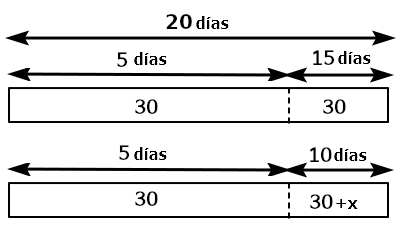
\includegraphics[width=\linewidth]{../images/tableS8L103_agri}
        \end{figure}
    \end{minipage}\hfill
    \begin{minipage}{.55\textwidth}
        Observamos que, en esta situación, a mayor cantidad de agricultores, menos días se necesitarán para terminar la siembra.
        \begin{table}[H]
            \centering
            \begin{tabular}{|l|c|l|}
                \hline
                Cantidad de agricultores    & 30 & 30+x \\
                \hline
                Cantidad de días de trabajo & 15 & 10   \\
                \hline
            \end{tabular}
        \end{table}
        Como es una relación inversamente proporcional, planteamos la siguiente relación:
        \begin{align*}
            30 \times 15 & = 10 \times (30+x) \\
            450          & = 300 +10x         \\
            10x          & = 450-300          \\
            10x          & = 150              \\
            x            & = 15
        \end{align*}
    \end{minipage}

    En el segundo grupo, había 15 agricultores más, es decir, un total de 45 agricultores.
\end{solutionbox}